\documentclass{ximera}

%% You can put user macros here
%% However, you cannot make new environments

\listfiles

\graphicspath{{./}{firstExample/}{secondExample/}}

\usepackage{tikz}
\usepackage{tkz-euclide}
\usepackage{tikz-3dplot}
\usepackage{tikz-cd}
\usetikzlibrary{shapes.geometric}
\usetikzlibrary{arrows}
\usetikzlibrary{decorations.pathmorphing,patterns}
\usetkzobj{all}
\pgfplotsset{compat=1.13} % prevents compile error.

\renewcommand{\vec}[1]{\mathbf{#1}}
\newcommand{\RR}{\mathbb{R}}
\newcommand{\dfn}{\textit}
\newcommand{\dotp}{\cdot}
\newcommand{\id}{\text{id}}
\newcommand\norm[1]{\left\lVert#1\right\rVert}
 
\newtheorem{general}{Generalization}
\newtheorem{initprob}{Exploration Problem}

\tikzstyle geometryDiagrams=[ultra thick,color=blue!50!black]

\usepackage{mathtools}

\title{Transformation of Homogeneous Equations into Separable Equations}%\label{Module 2-A}

\begin{document}

\begin{abstract}
Need an abstract
\end{abstract}

\maketitle

% \title{Transformation of Nonlinear Equations into Separable Equations}


% In Module \ref{Module 1-B} we learned how to solve the first-order linear
% equation
% $$
% y'+p(x)y=f(x)
% $$


% are of the form $y=uy_1$, where $y_1$ is a nontrivial solution of the
% complementary equation
% \begin{equation} \label{eq:2.4.1}
% y'+p(x)y=0
% \end{equation}
% and $u$ is a solution of
% $$
% u'y_1(x)=f(x).
% $$
% Note that this last equation is separable, since it can be rewritten
% as
% $$
% u'={f(x)\over y_1(x)}.
% $$
% In this section we'll consider nonlinear differential equations
% that are not separable to begin with, but can be solved in a similar
% fashion by writing their solutions in the form $y=uy_1$, where $y_1$
% is a suitably chosen known function and $u$ satisfies a separable
% equation. We'll say in this case  that we \dfn{transformed} the given equation into a separable equation.

% \section*{Bernoulli Equations}
% \noindent
% A \href{http://www-history.mcs.st-and.ac.uk/Mathematicians/Bernoulli_Jacob.html}
% \dfn{Bernoulli equation} is an equation  of
% the form
% \begin{equation} \label{eq:2.4.2}
% y'+p(x)y=f(x)y^r,
% \end{equation}
% where $r$ can be any real number other than $0$ or $1$. (Note that
% \eqref{eq:2.4.2} is linear if and only if $r=0$ or $r=1$.) 

% We can
% transform
% \eqref{eq:2.4.2} into a separable equation by variation of parameters:
% if  $y_1$ is  a nontrivial solution of \eqref{eq:2.4.1},
% substituting
% $y=uy_1$ into \eqref{eq:2.4.2} yields
% $$
% u'y_1+u(y_1'+p(x)y_1)=f(x)(uy_1)^r,
% $$
% which is equivalent to the separable equation
% $$
% u'y_1(x)=f(x)\left(y_1(x)\right)^ru^r\mbox{\quad or \quad}
% {u'\over u^r}=f(x)\left(y_1(x)\right)^{r-1},
% $$
% since $y_1'+p(x)y_1=0$.

% \begin{example}\label{example:2.4.1}
% Solve the Bernoulli equation
% \begin{equation} \label{eq:2.4.3}
% y'-y=xy^2.
% \end{equation}
% \end{example}

% \solution
% Since $y_1=e^x$ is a solution of $y'-y=0$, we look for solutions of
% \eqref{eq:2.4.3}  in the form $y=ue^x$, where
% $$
% u'e^x=xu^2e^{2x}\mbox{\quad or, equivalently, \quad}
% u'=xu^2e^x.
% $$
% Separating variables yields
% $$
% {u'\over u^2}=xe^x,
% $$
% and integrating yields
% $$
% -{1\over u}=(x-1)e^x+c.
% $$
% Hence,
% $$
% u=-{1\over(x-1)e^x+c}
% $$
% and
% $$
% y=-{1\over x-1+ce^{-x}}.
% $$

% Figure~\ref{eq:2.4.1}  shows
%  direction field and some integral curves of \eqref{eq:2.4.3}.


% \begin{figure}[tbp]
%   \centering
%   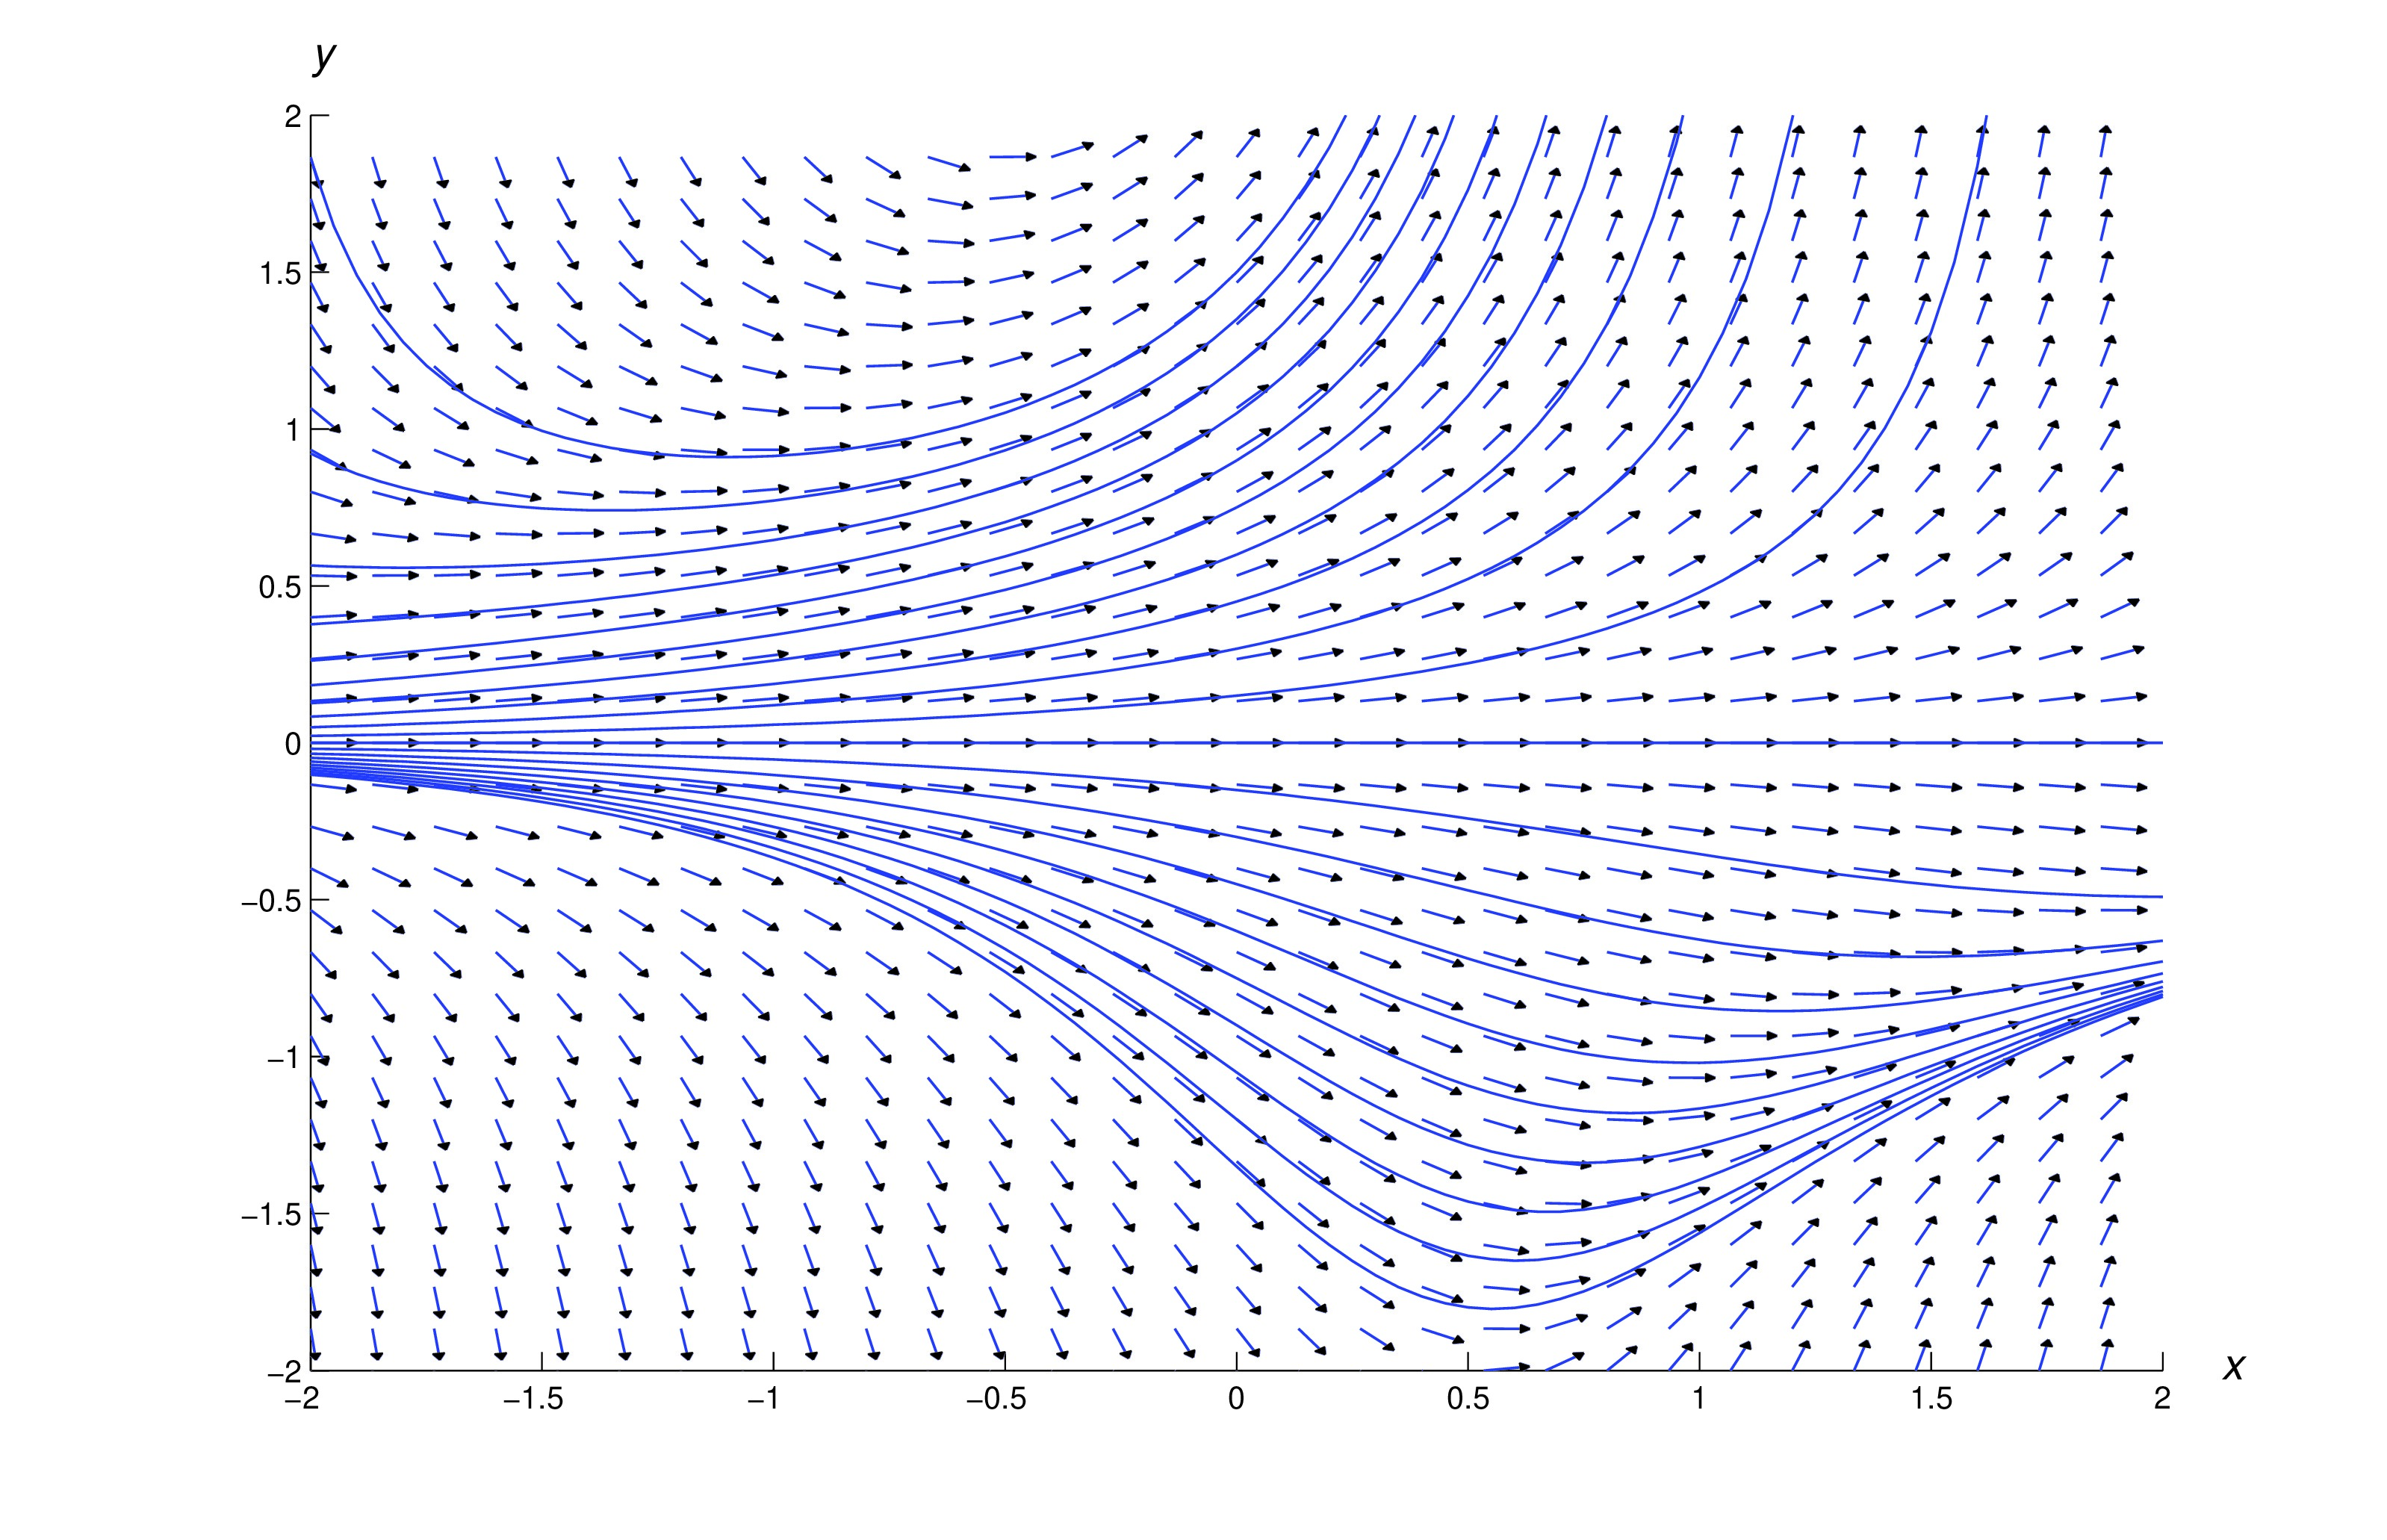
\includegraphics[bb=-78 148 689 643,width=5.67in,height=3.66in,keepaspectratio]{fig020401}
% \color{blue}
% \caption{A direction field and integral curves for $y'-y=xy^{2}$}
%   \label{figure:2.4.1}
% \end{figure}

\section*{Transformation of Homogeneous Equations into Separable Equations}
\subsection*{Nonlinear Equations That Can be  Transformed Into Separable Equations}

We've seen that the nonlinear Bernoulli equation can be transformed
into a separable equation by  the substitution $y=uy_1$ if
$y_1$ is suitably chosen. Now let's discover a sufficient condition
for a nonlinear first order differential equation
\begin{equation} \label{eq:2.4.4}
y'=f(x,y)
\end{equation}
to be transformable into a separable equation in the same way.
  Substituting $y=uy_1$  into
\eqref{eq:2.4.4} yields
$$
u'y_1(x)+uy_1'(x)=f(x,uy_1(x)),
$$
which is equivalent to
\begin{equation} \label{eq:2.4.5}
u'y_1(x)=f(x,uy_1(x))-uy_1'(x).
\end{equation}
If
$$
f(x,uy_1(x))=q(u)y_1'(x)
$$
for some function $q$, then   \eqref{eq:2.4.5} becomes
\begin{equation} \label{eq:2.4.6}
u'y_1(x)=(q(u)-u)y_1'(x),
\end{equation}
which is separable. After checking for constant solutions $u\equiv
u_0$ such that $q(u_0)=u_0$, we can separate
variables to obtain
$$
\frac{u'}{q(u)-u}=\frac{y_1'(x)}{y_1(x)}.
$$

\subsection*{Homogeneous Nonlinear Equations}

In the text  we'll consider only the most widely studied class of
equations for which the method of the preceding paragraph works.
Other types of equations appear in
Exercises~\ref{exer:2.4.44}--\ref{exer:2.4.51}.

The differential equation \eqref{eq:2.4.4}
is said to be \dfn{homogeneous} if  $x$ and $y$
occur in $f$ in such a way that  $f(x,y)$ depends only
on the ratio $y/x$; that is, \eqref{eq:2.4.4} can be written as
\begin{equation} \label{eq:2.4.7}
y'=q(y/x),
\end{equation}
where $q=q(u)$ is a function of a single variable.
For example,
$$
y'=\frac{y+xe^{-y/x}}{x}=\frac{y}{x}+e^{-y/x}
$$
and
$$
y'=\frac{y^2+xy-x^2}{x^2}=\left(\frac{y}{x}\right)^2+\frac{y}{x}
-1
$$
are of the form  \eqref{eq:2.4.7}, with
$$
q(u)=u+e^{-u}\quad\text{and}\quad q(u)=u^2+u-1,
$$
respectively. The general method discussed above can be
applied to
\eqref{eq:2.4.7} with $y_1=x$ (and therefore $y_1'=1)$. Thus,
substituting $y=ux$ in \eqref{eq:2.4.7} yields
$$
u'x+u=q(u),
$$
and separation of variables (after checking for constant
solutions $u\equiv u_0$ such that $q(u_0)=u_0$) yields
$$
\frac{u'}{q(u)-u}=\frac{1}{x}.
$$

Before turning to examples, we point out something that you may've have
already noticed:
 the definition of \dfn{homogeneous equation} given
here isn't  the same as the definition given in {\color{red} Section~2.1},
where we said that a linear equation of the form
$$
y'+p(x)y=0
$$
is homogeneous. We make no apology for this inconsistency, since we
didn't create it!  Historically, \dfn{homogeneous} has been
used in these two inconsistent ways. The one
having to do with linear equations is the most important. This
is the only section of the book where the meaning defined here will
apply.

Since $y/x$ is in general undefined if $x=0$, we'll consider
solutions of nonhomogeneous equations only on open intervals that do
not contain the point $x=0$.

\begin{example}\label{example:2.4.2}
Solve
\begin{equation} \label{eq:2.4.8}
y'=\frac{y+xe^{-y/x}}{x}.
\end{equation}
\end{example}

% Commented out by Felipe
%\solution 
Substituting  $y=ux$
into \eqref{eq:2.4.8} yields
$$
u'x+u =  \frac{ux+xe^{-ux/x}}{x} = u+e^{-u}.
$$
 Simplifying and separating variables yields
$$
e^uu'=\frac{1}{x}.
$$
Integrating yields
$e^u=\ln |x|+c$.
Therefore
$u=\ln(\ln|x|+c)$ and
$y=ux=x \ln (\ln |x|+c)$.

Figure~\ref{figure:2.4.2} shows
a direction field and integral curves for \eqref{eq:2.4.8}.


\begin{image}
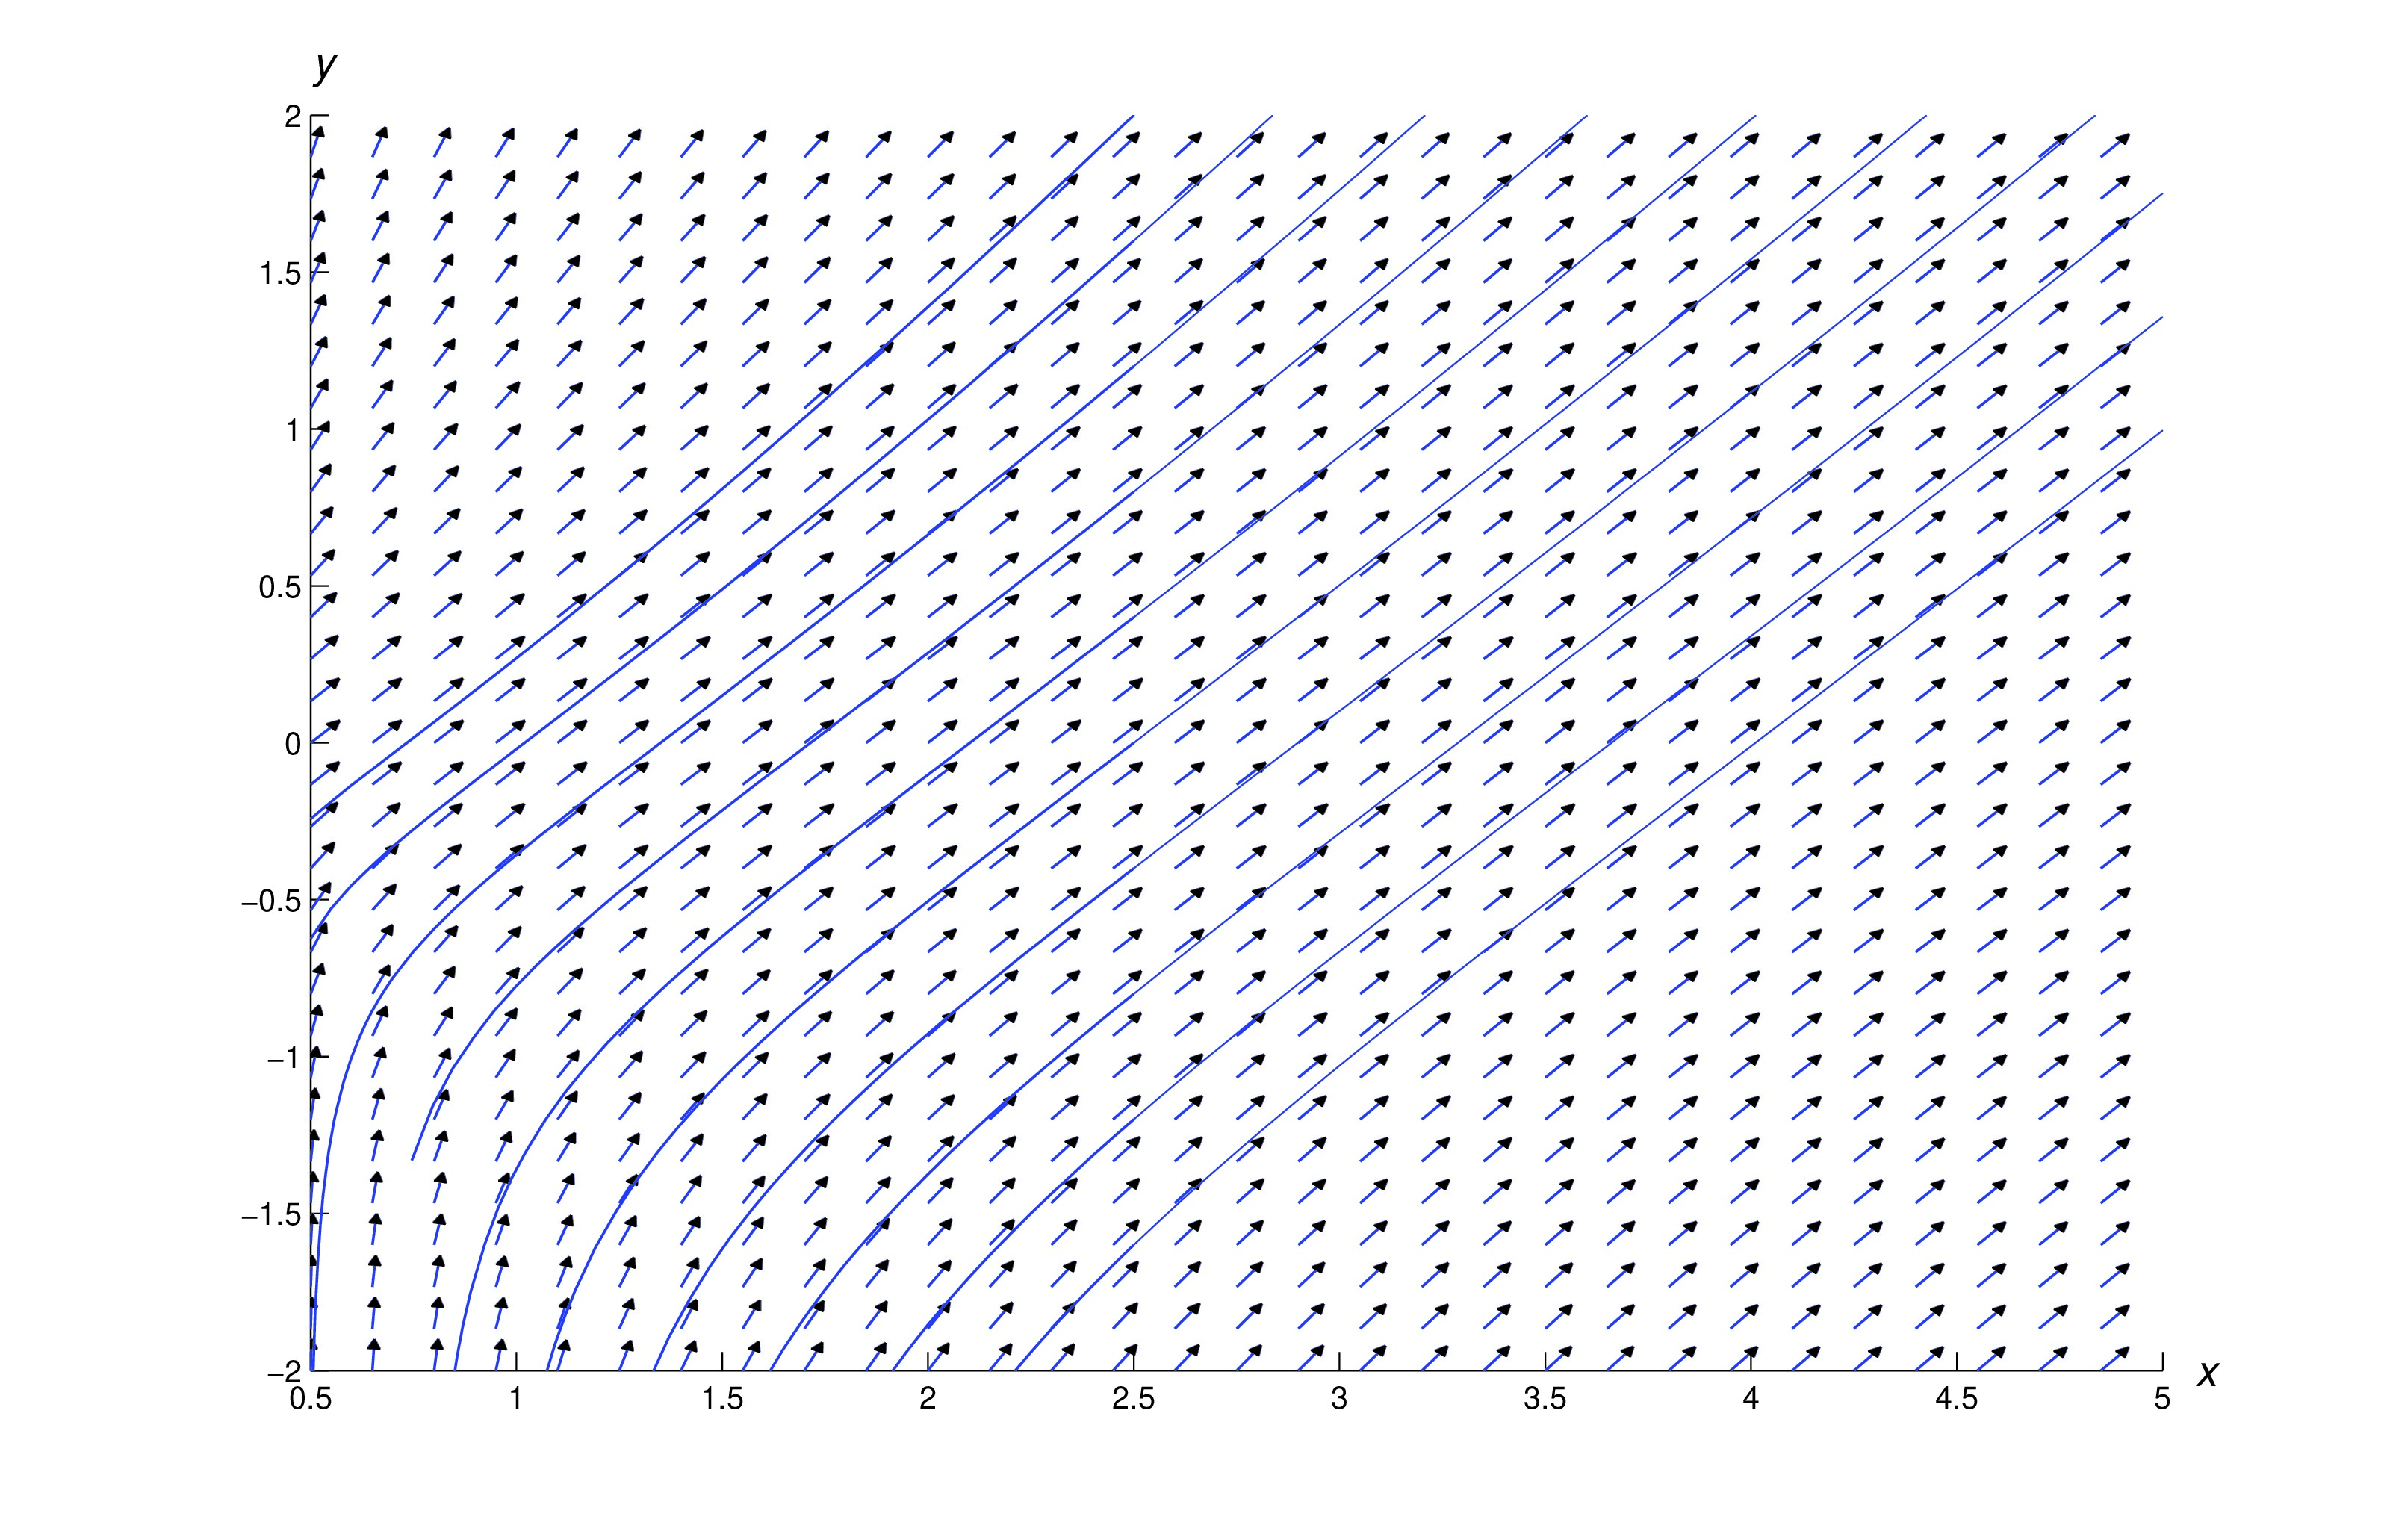
\includegraphics[height=1.5in]{fig020402.jpg}
\end{image}
\begin{center}
\begin{figure}
%  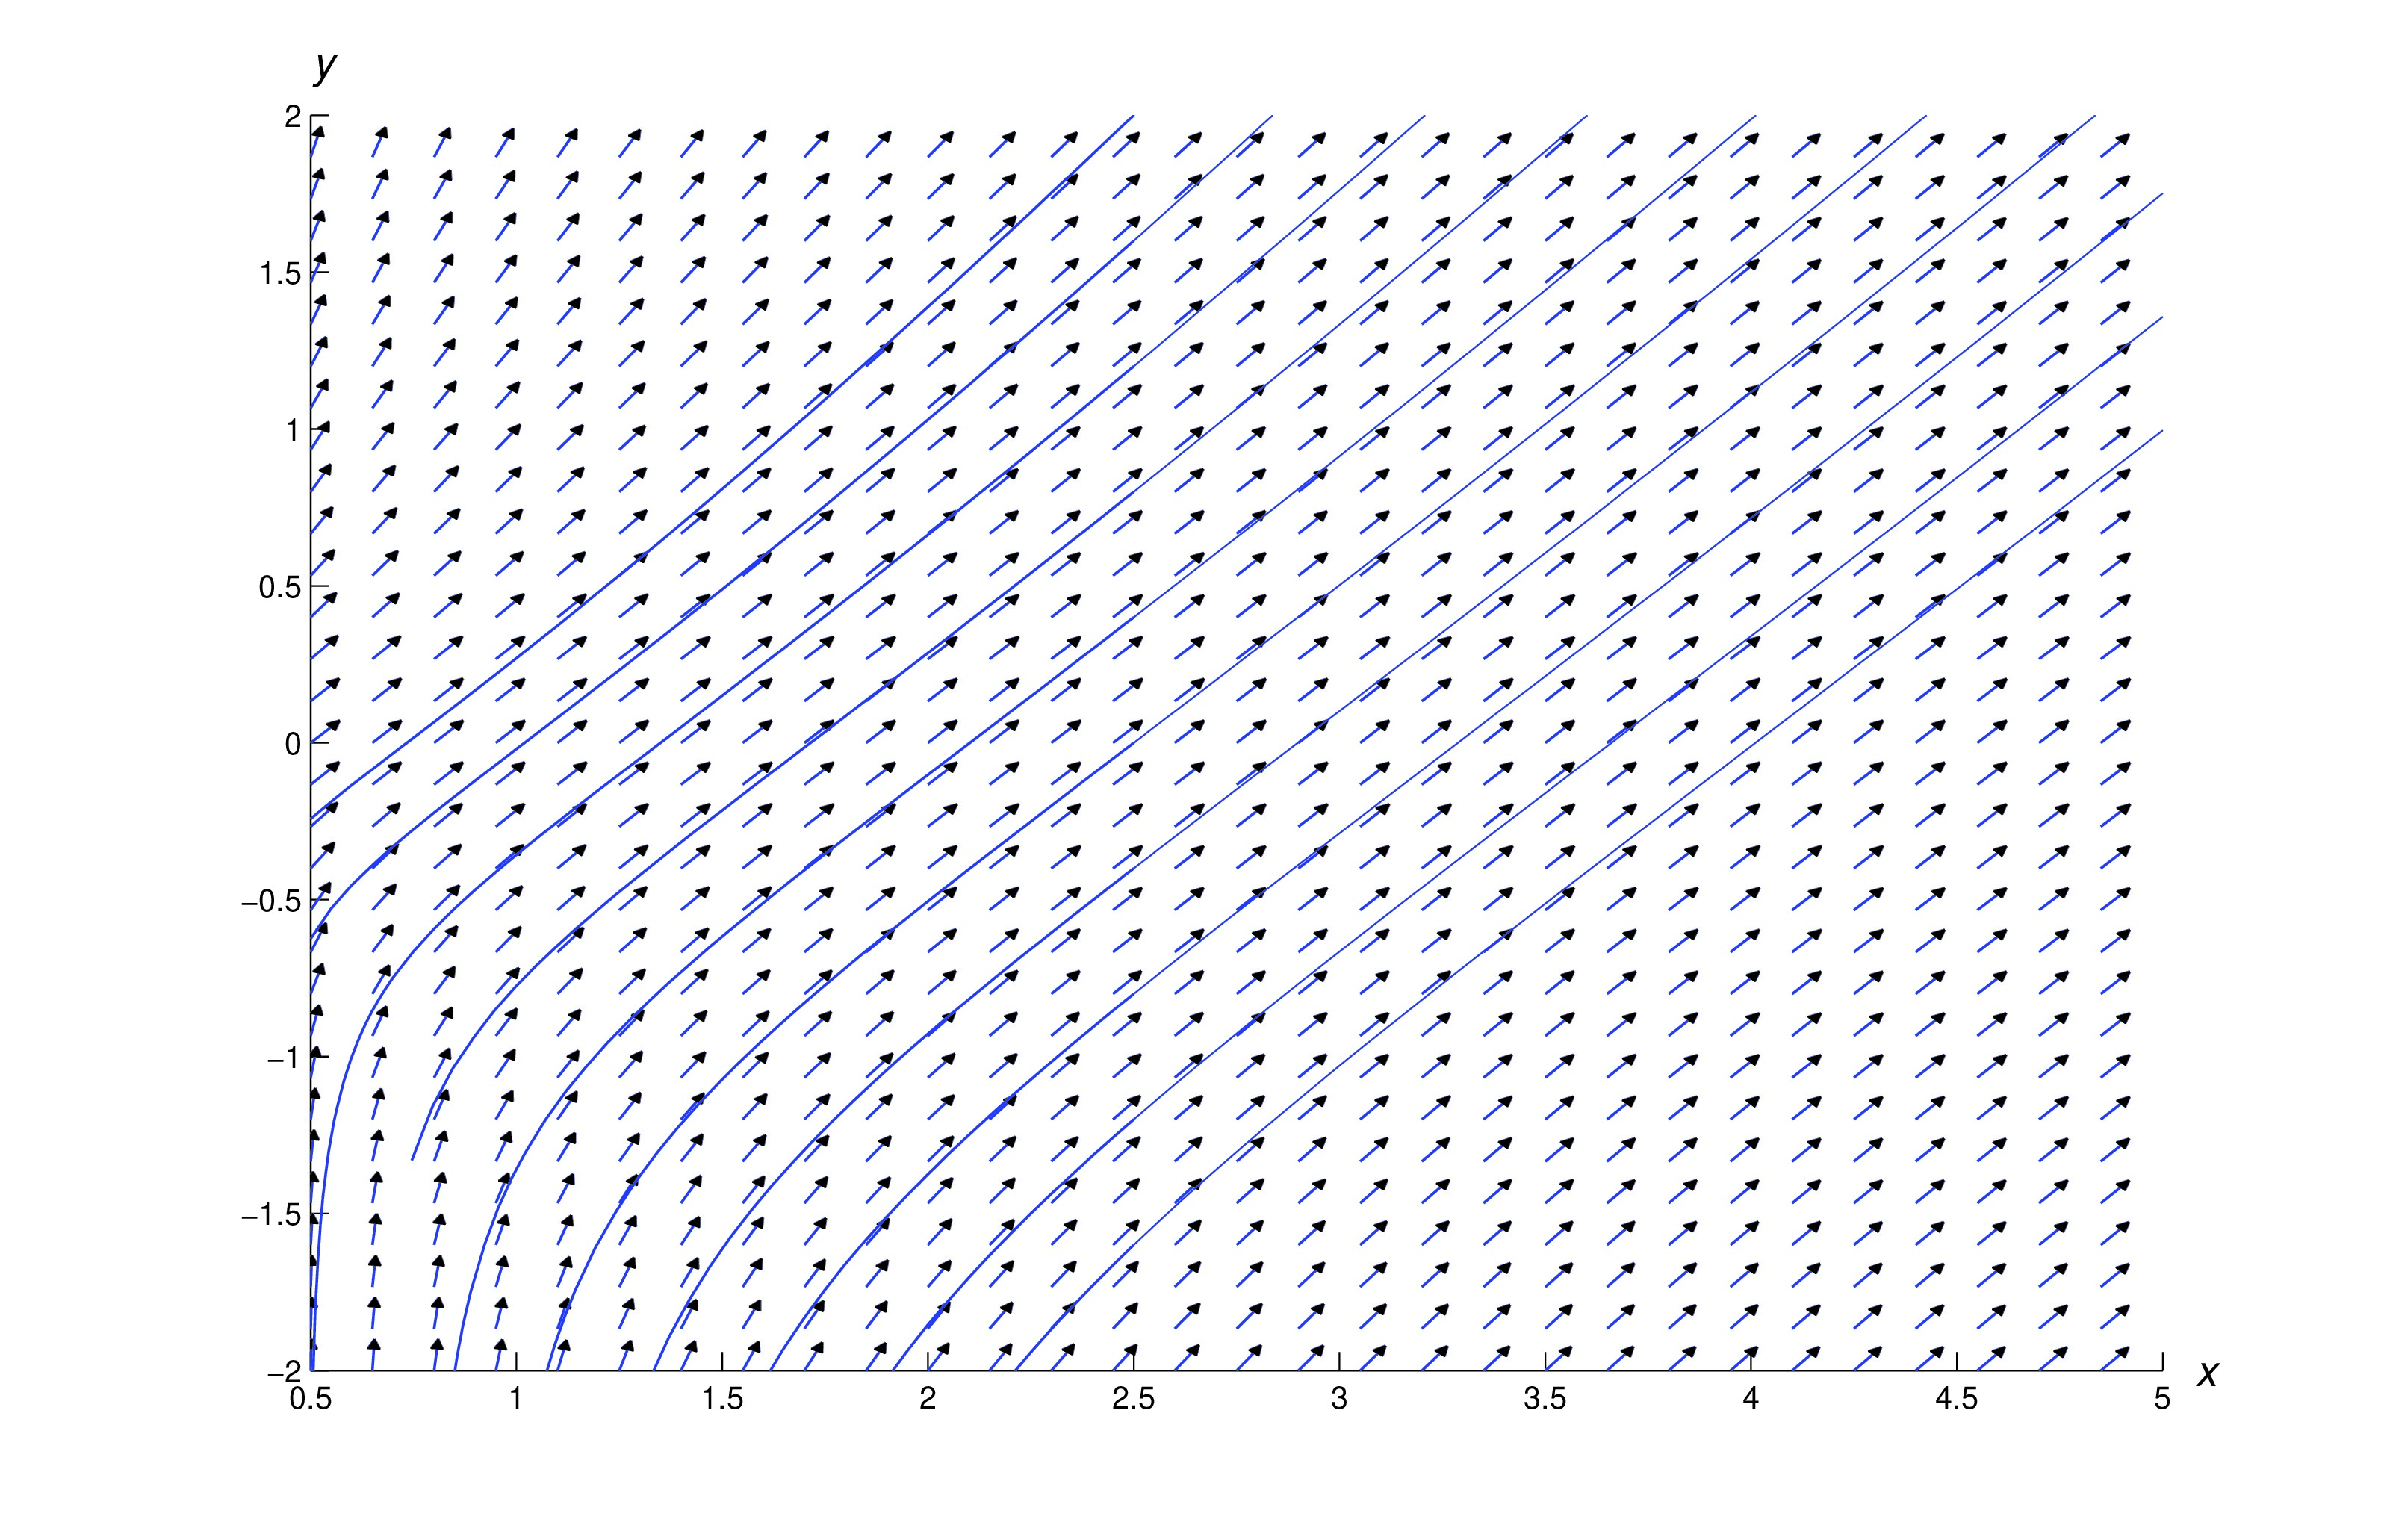
\includegraphics[bb=-78 148 689 643,width=5.67in,height=3.66in,keepaspectratio]{fig020402}
\caption
{A direction field and some integral curves for
$y'=\frac{y+xe^{-y/x}}{x}$}
  \label{figure:2.4.2}
\end{figure}
\end{center}

\begin{example}\label{example:2.4.3}

\begin{enumerate}
\item\label{example:2.4.3a} %(a)
Solve
\begin{equation} \label{eq:2.4.9}
x^2y'=y^2+xy-x^2.
\end{equation}

\item\label{example:2.4.3b} %(b)
Solve the initial value problem
\begin{equation} \label{eq:2.4.10}
x^2y'=y^2+xy-x^2, \quad y(1)=2.
\end{equation}
\end{enumerate}

\begin{explanation}
\ref{example:2.4.3a} We first find solutions of \eqref{eq:2.4.9} on open intervals that don't
contain $x=0$. We can rewrite \eqref{eq:2.4.9} as
$$
y'=\frac{y^2+xy-x^2}{x^2}
$$
for $x$ in any such interval. Substituting $y=ux$ yields
$$
u'x+u =\frac{(ux)^2+x(ux)-x^2}{x^2}
= u^2+u-1,
$$
so
\begin{equation} \label{eq:2.4.11}
u'x=u^2-1.
\end{equation}
By inspection this equation has the constant solutions $u\equiv1$ and
$u\equiv-1$. Therefore $y=x$ and $y=-x$ are solutions of
\eqref{eq:2.4.9}. If $u$ is a solution of \eqref{eq:2.4.11} that doesn't
assume the values $\pm 1$ on some interval,  separating variables
yields
$$
\frac{u'}{u^2-1}=\frac{1}{x},
$$
 or, after a partial fraction expansion,
$$
{\frac{1}{2}}\left[\frac{1}{u-1}-\frac{1}{u+1}\right]u'=
\frac{1}{x}.
$$
 Multiplying by 2 and integrating yields
$$
\ln\left|\frac{u-1}{u+1}\right| =2 \ln |x|+k,
$$
 or
$$
\left|\frac{u-1}{u+1}\right||=e^kx^2,
$$
which holds if
\begin{equation} \label{eq:2.4.12}
\frac{u-1}{u+1}=cx^2
\end{equation}
where $c$ is an arbitrary constant.
  Solving for $u$ yields
$$
u =\frac{1+cx^2}{1-cx^2}.
$$
\begin{image}
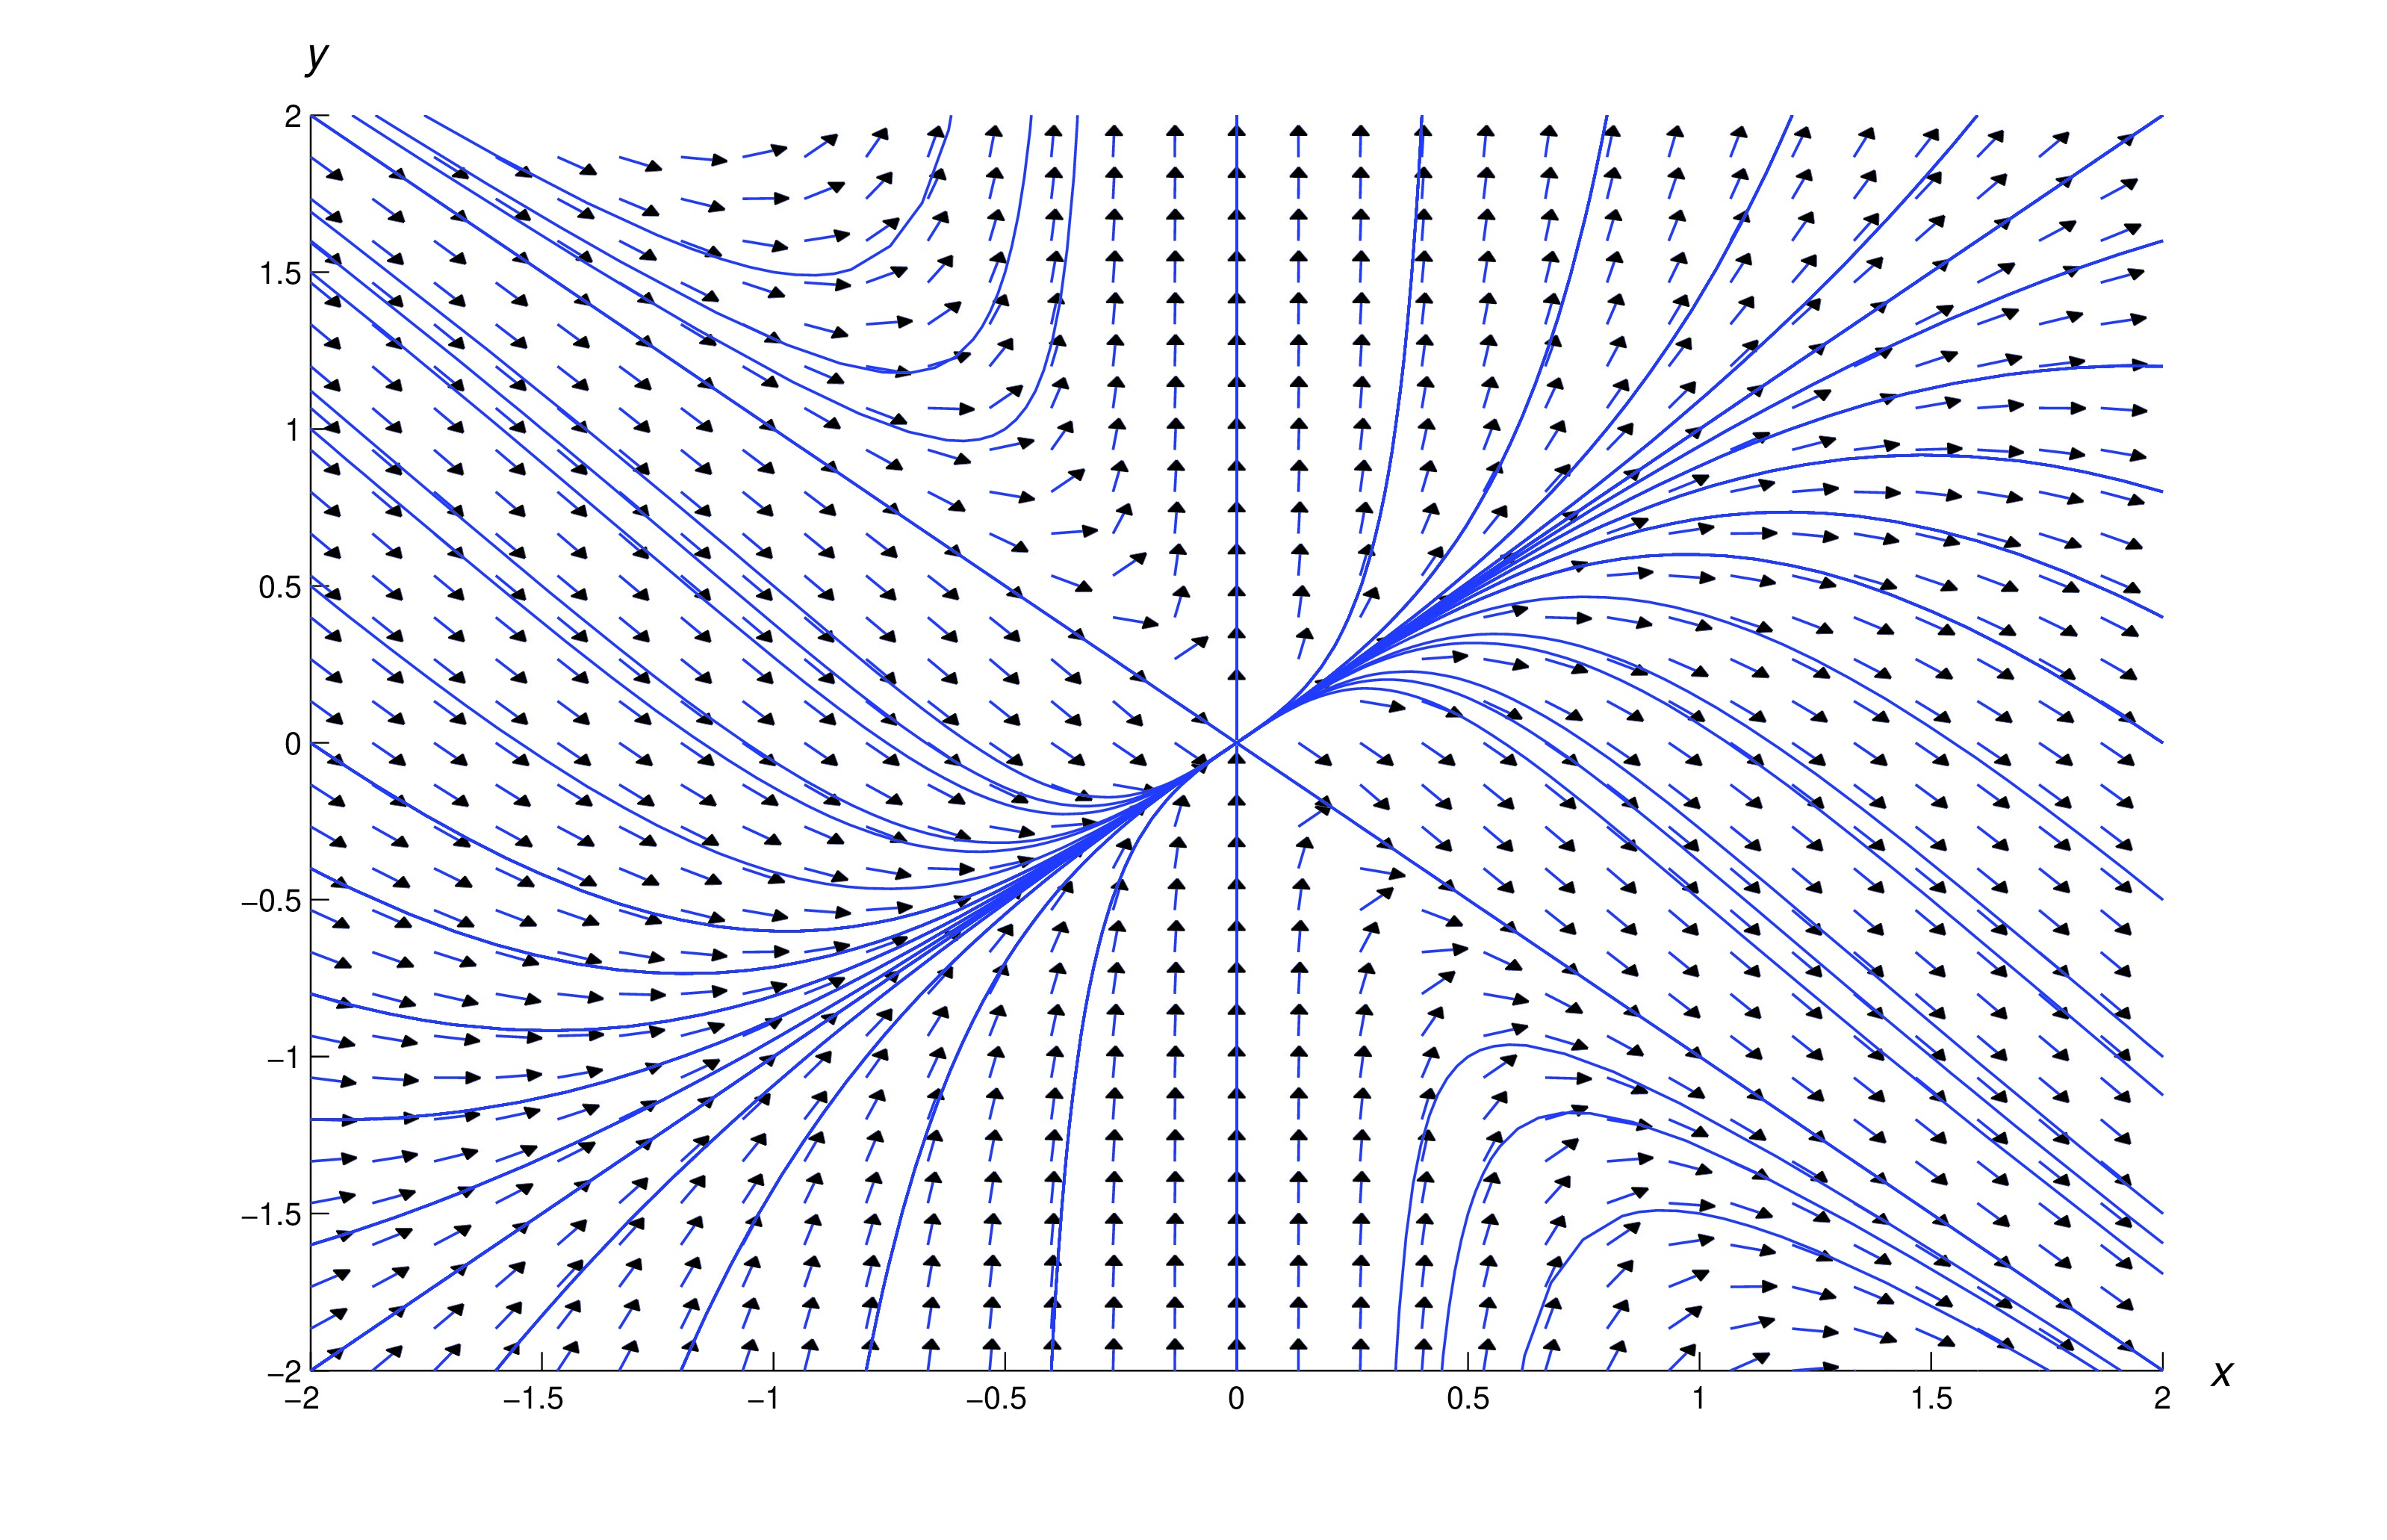
\includegraphics[height=1.5in]{fig020403.jpg} 
\end{image}
\begin{center}
\begin{figure}
%  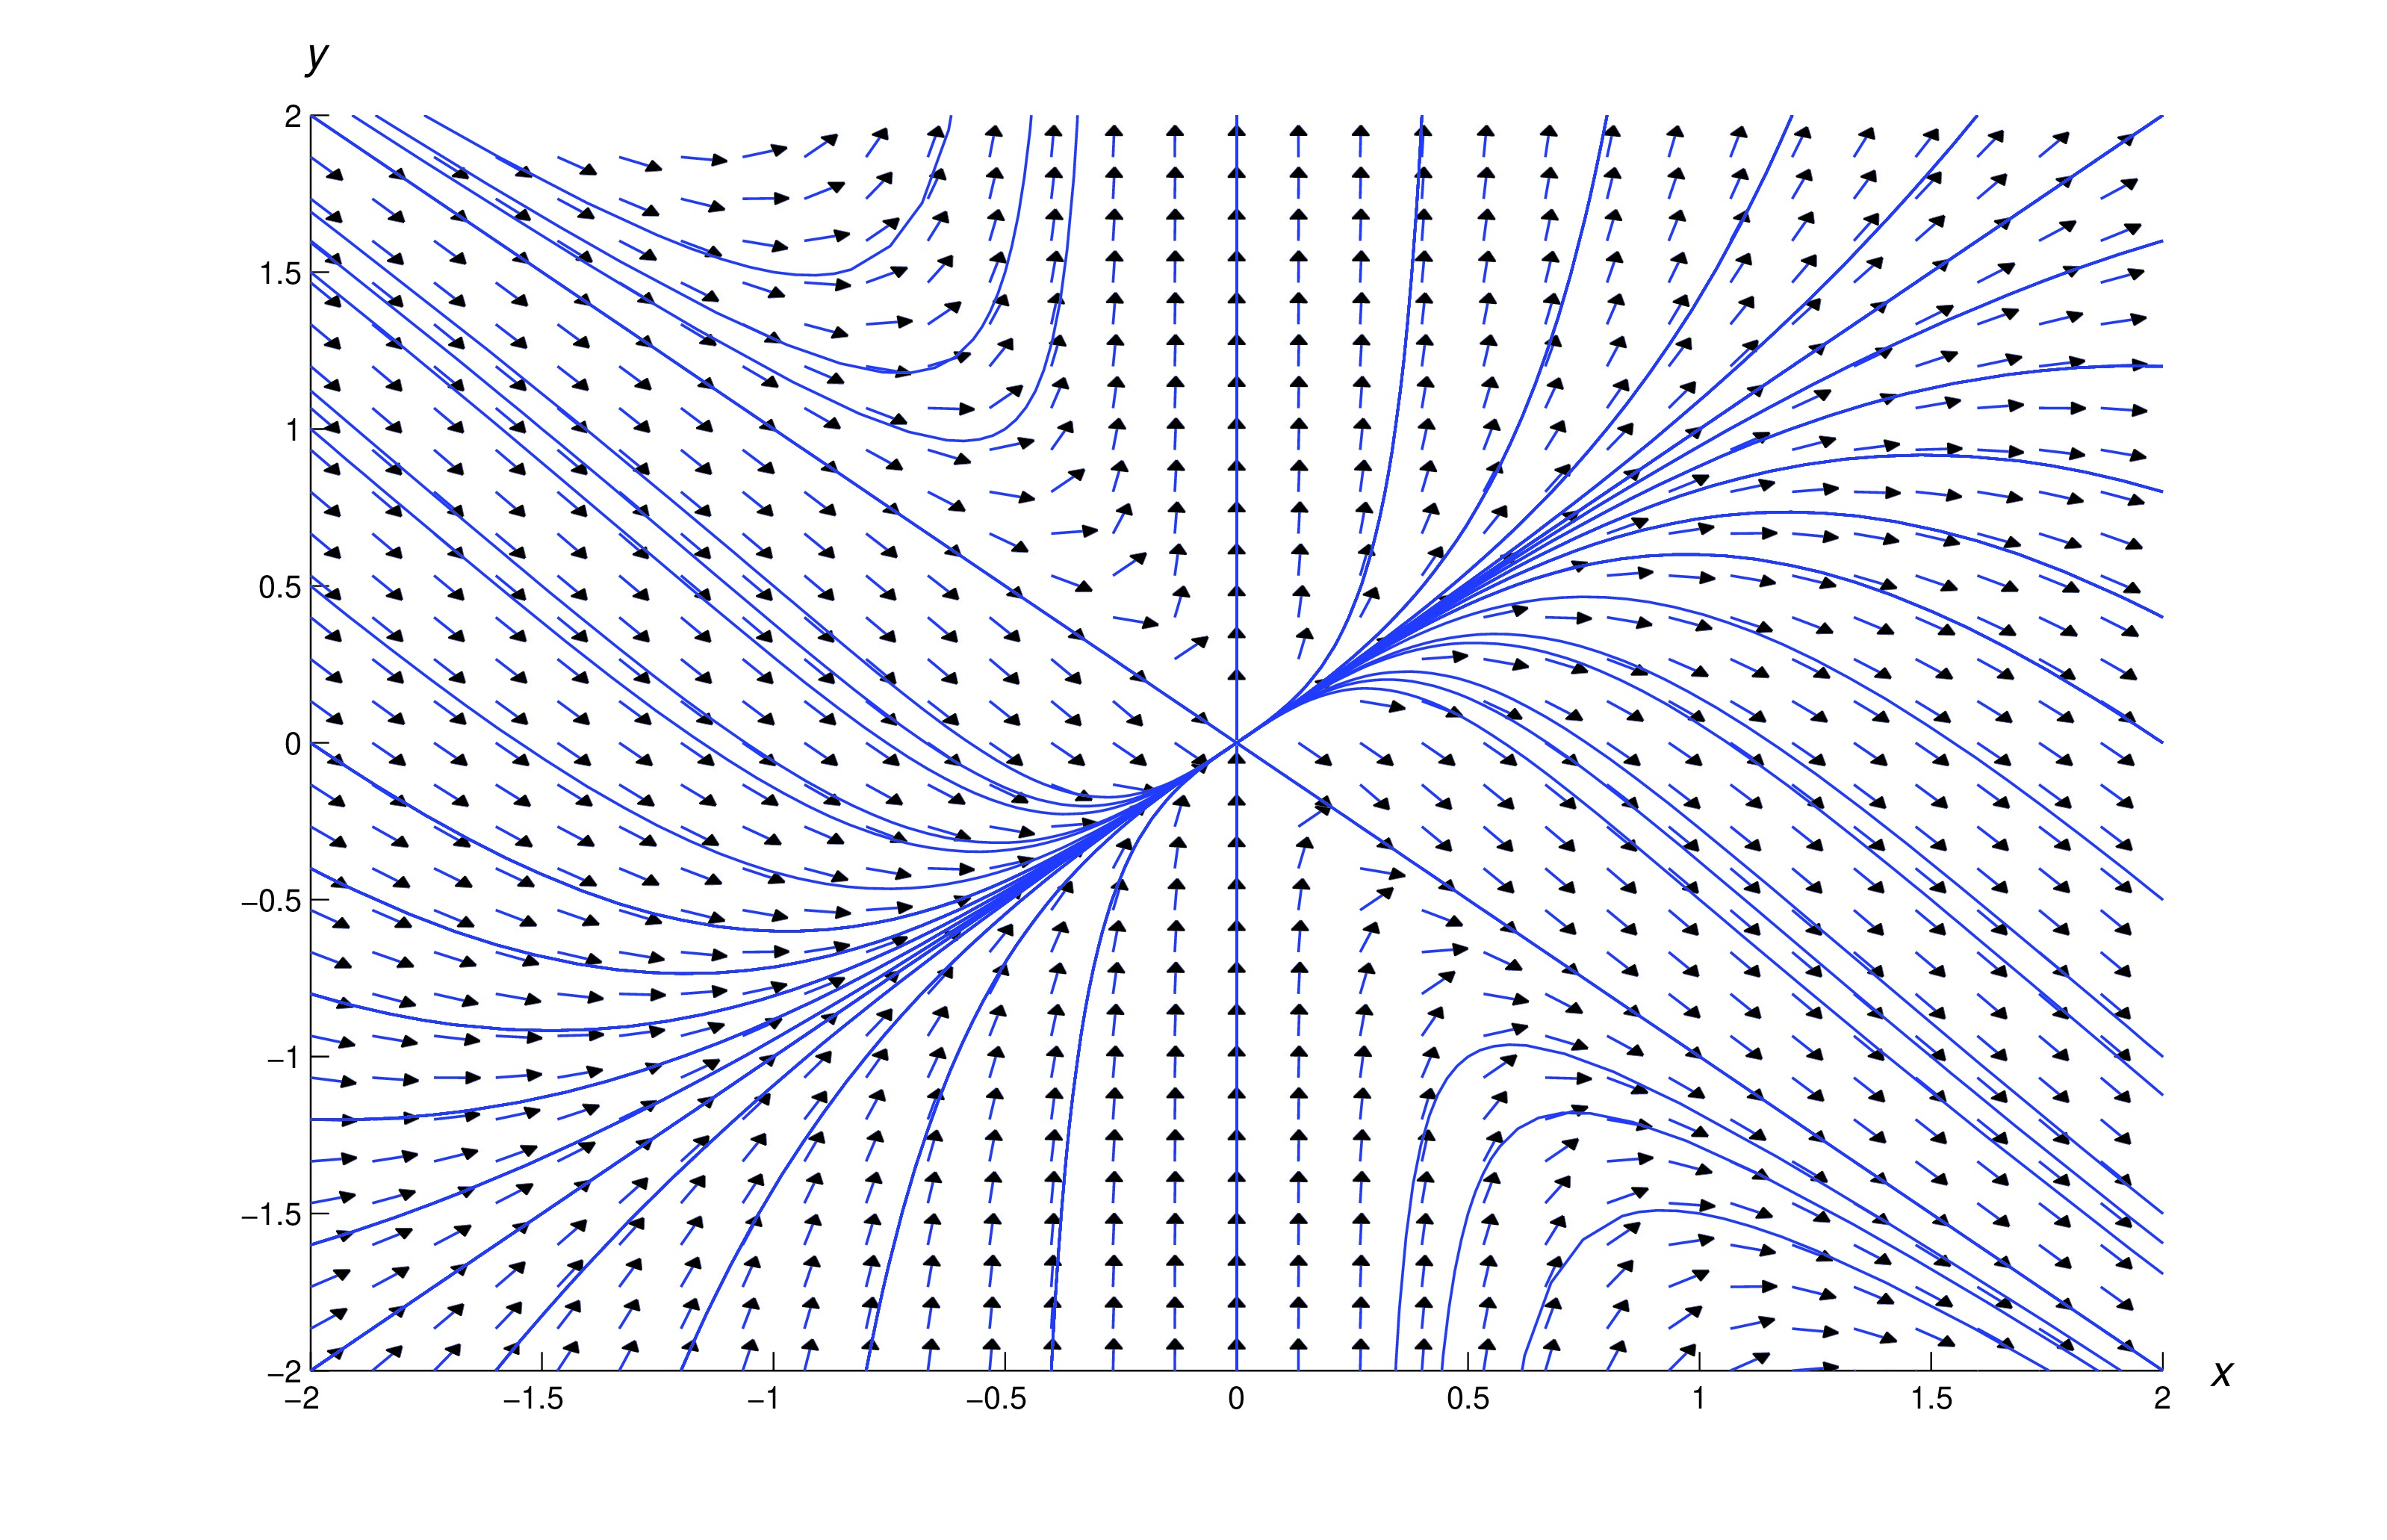
\includegraphics[bb=-78 148 689 643,width=5.67in,height=3.66in,keepaspectratio]{fig020403} }
\caption{A direction field and  integral curves for
$x^{2}y'=y^{2}+xy-x^{2}$}
  \label{figure:2.4.3}
  \end{figure}
  \end{center}
  
  \begin{image}
  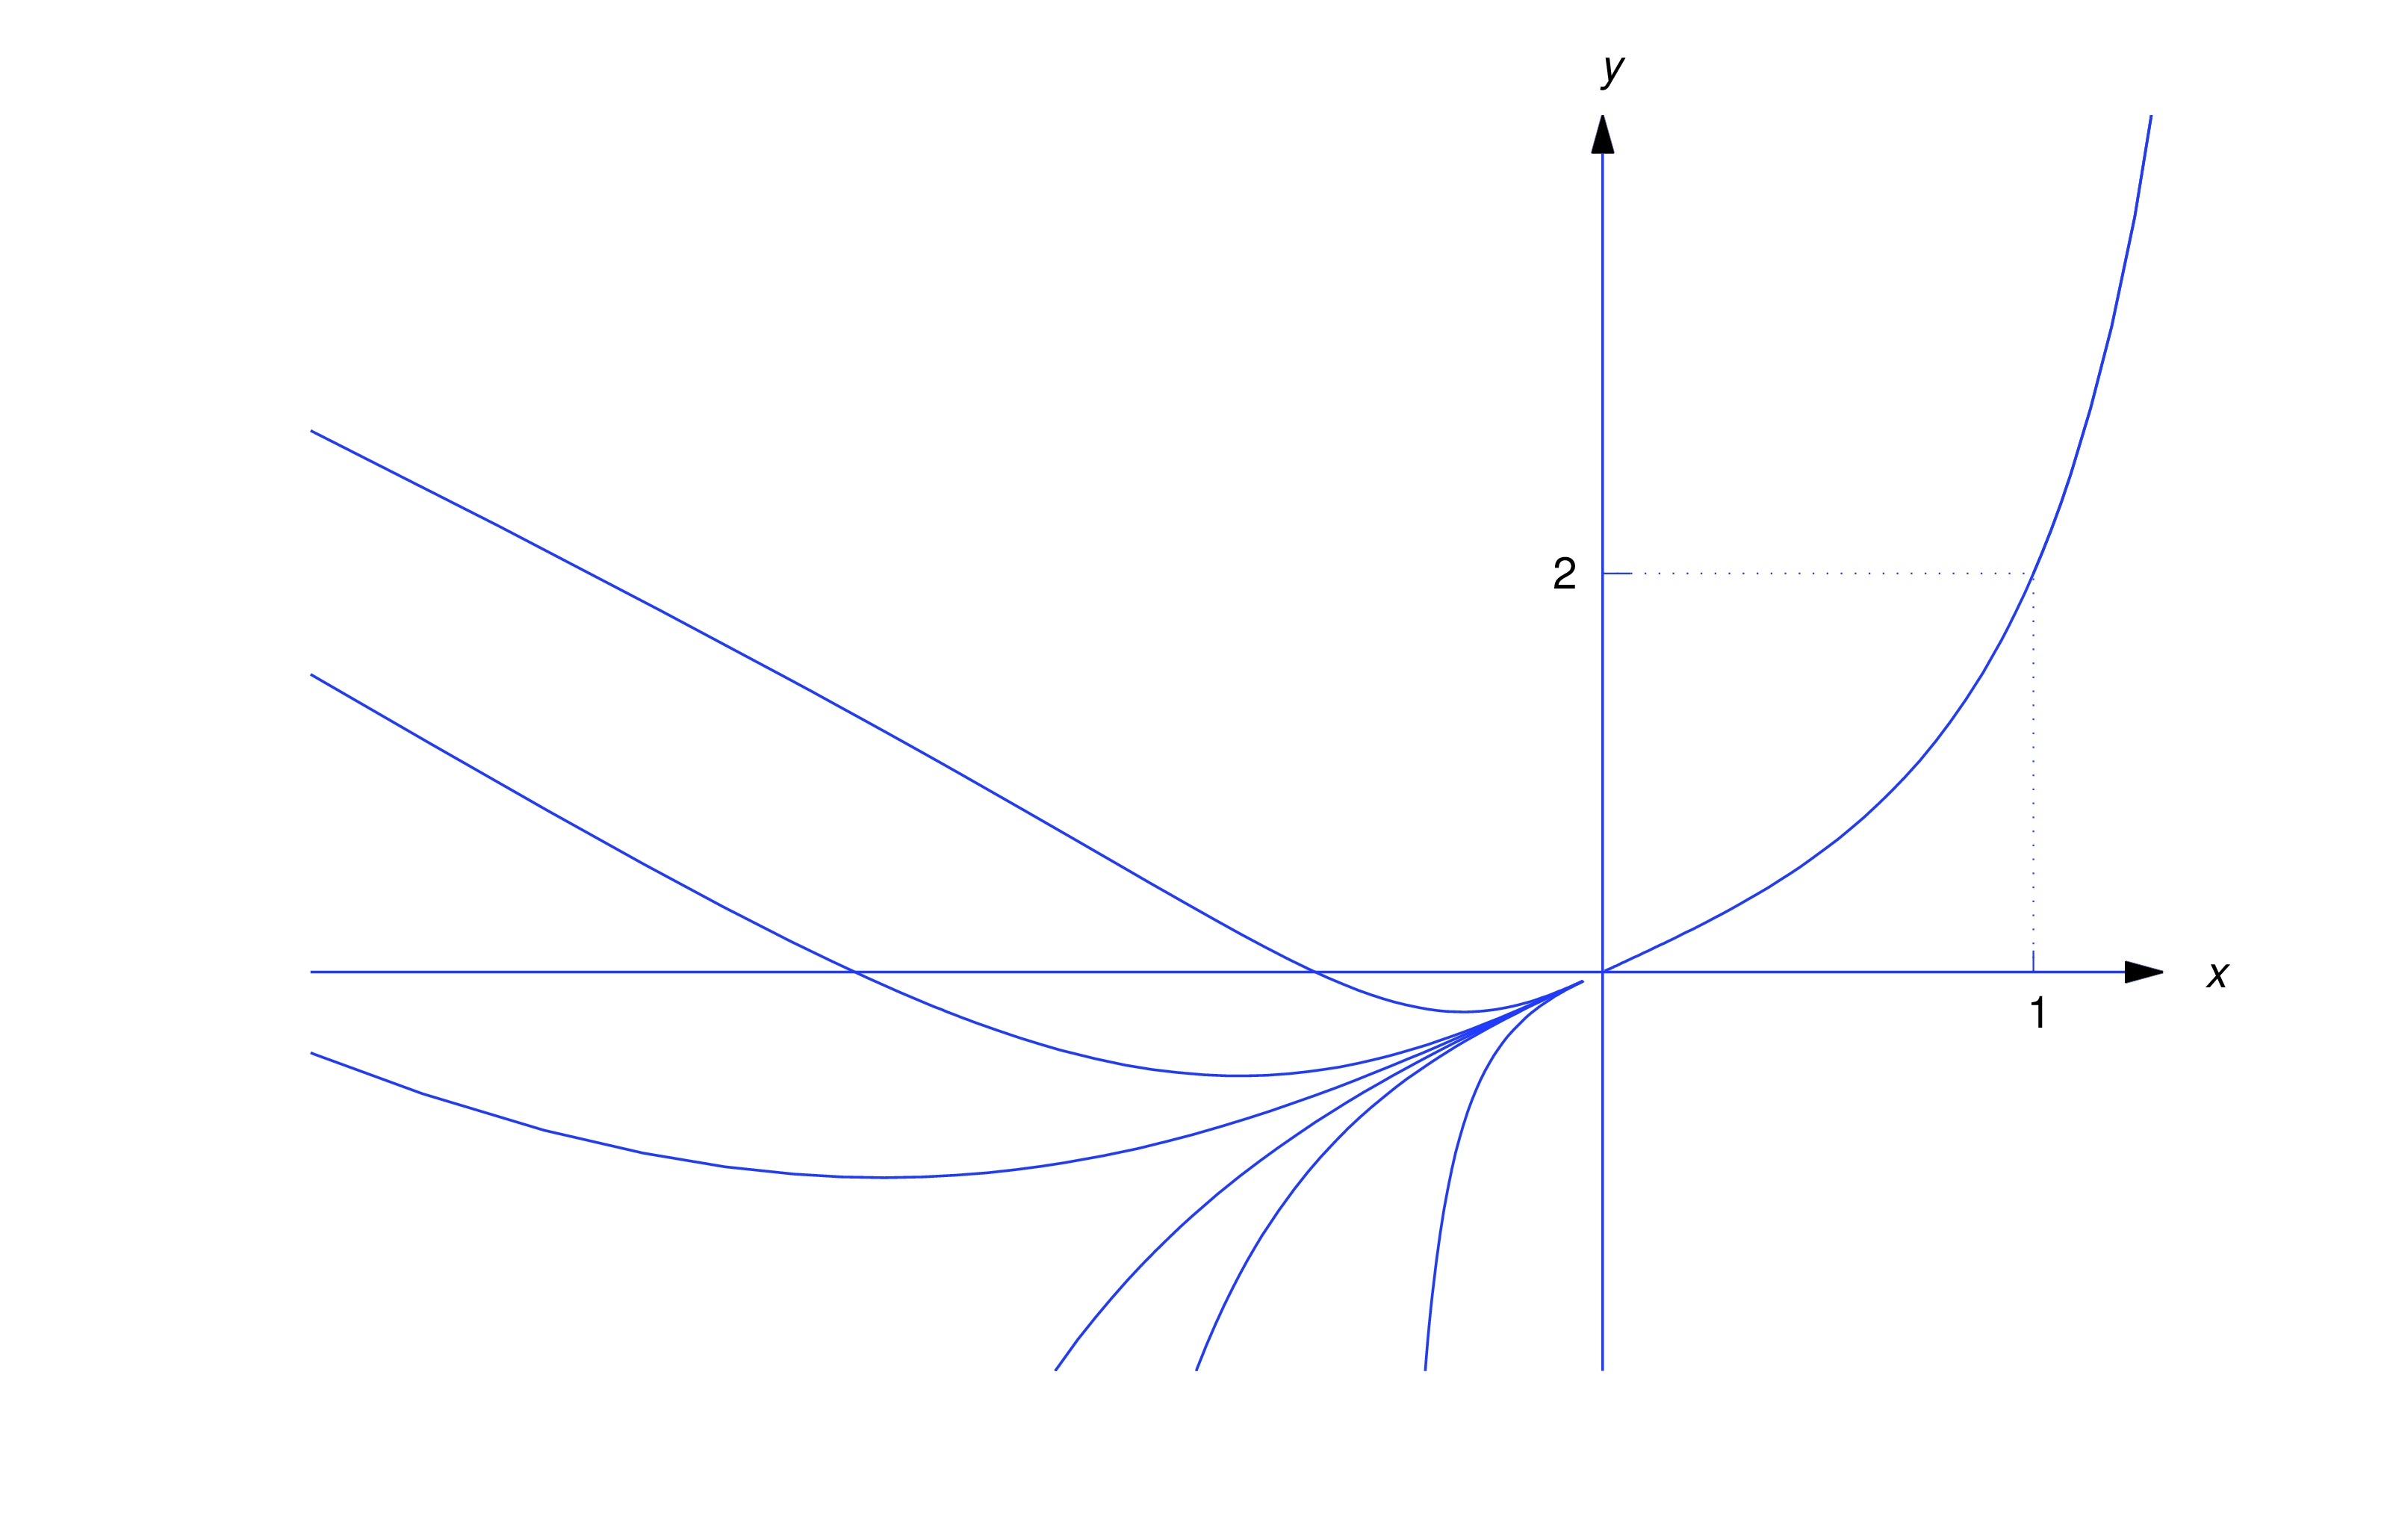
\includegraphics[height=1.5in]{fig020404.jpg}
  \end{image}
  
  \begin{center}
  \begin{figure}
\caption{Solutions of  $x^{2}y'=y^{2}+xy-x^{2}$, $y(1)=2$}
  \label{figure:2.4.4}
 \end{figure}
\end{center}

Therefore
\begin{equation} \label{eq:2.4.13}
y=ux=\frac{x(1+cx^2)}{1-cx^2}
\end{equation}
is a solution of \eqref{eq:2.4.10} for any choice of the constant $c$.
Setting $c=0$ in \eqref{eq:2.4.13} yields the solution $y=x$. However, the
solution $y=-x$ can't be obtained from \eqref{eq:2.4.13}. Thus, the
solutions of \eqref{eq:2.4.9} on intervals that don't contain $x=0$ are
$y=-x$ and functions of the form \eqref{eq:2.4.13}.

The situation is more complicated if $x=0$ is the open interval.
 First, note that $y=-x$ satisfies \eqref{eq:2.4.9}
on $(-\infty,\infty)$. If $c_1$ and $c_2$ are arbitrary constants,
 the function
\begin{equation} \label{eq:2.4.14}
y=\left\{\begin{array}{ll} \frac{x(1+c_1x^2)}{1-c_1x^2},&a<x<0,\\
\frac{x(1+c_2x^2)}{1-c_2x^2},&0\leq x<b,
 \end{array}\right.
\end{equation}
is a solution of \eqref{eq:2.4.9} on $(a,b)$, where
$$
a=\left\{\begin{array}{cl}-\frac{1}{\sqrt{c_1}}&\text{ if }c_1>0,\\
-\infty&\text{ if }c_1\leq 0,
\end{array}\right. \quad\text{and}\quad
b=\left\{\begin{array}{cl}\frac{1}{\sqrt{c_2}}&\text{ if }c_2>0,\\
\infty&\text{ if }c_2\leq 0.
\end{array}\right.
$$
We leave it to you to verify this. To do so, note that if $y$ is
any function of the form \eqref{eq:2.4.13} then $y(0)=0$ and $y'(0)=1$.


Figure~\ref{figure:2.4.3} shows a direction field and some integral curves
for \eqref{eq:2.4.9}.



\ref{example:2.4.3b}  We could obtain $c$ by imposing
the initial condition $y(1)=2$ in \eqref{eq:2.4.13}, and then solving for
$c$. However, it's easier to use \eqref{eq:2.4.12}. Since $u=y/x$, the
initial
condition
$y(1)=2$ implies that $u(1)=2$.  Substituting this into \eqref{eq:2.4.12}
yields $c=1/3$.  Hence, the solution of \eqref{eq:2.4.10} is
$$
y=\frac{x(1+x^2/3)}{1-x^2/3}.
$$
The interval of validity of this solution is $(-\sqrt{3},\sqrt{3})$.
However, the largest interval on which \eqref{eq:2.4.10} has a unique
solution is $(0,\sqrt{3})$. To see this, note from \eqref{eq:2.4.14}
that any function of the form
\begin{equation} \label{eq:2.4.15}
y=\left\{\begin{array}{ll} \frac{x(1+cx^2)}{1-cx^2},&a<x\leq 0,\\
\frac{x(1+x^2/3)}{1-x^2/3},&0\leq x<\sqrt{3},
\end{array}\right.
\end{equation}
is a solution of \eqref{eq:2.4.10} on $(a,\sqrt{3})$, where $a=-1/\sqrt c$
if $c>0$ or $a=-\infty$ if $c\leq 0$. (Why doesn't this contradict
Theorem~\ref{thmtype:2.3.1}?)


 Figure~\ref{figure:2.4.4} shows several solutions of the
initial value problem~\eqref{eq:2.4.10}. Note that these solutions coincide
on $(0,\sqrt{3})$.
\end{explanation}
\end{example}

In the last two examples we were able to solve the given equations
explicitly.   However, this isn't  always possible, as you'll
see if you attempt the exercises in Trench, Section 2.4.
\end{document}